\newpage
\slidetitle{}
\section{Space Colonization Algorithmus\\}

\begin{itemize}
	\item Ursprünglich entwickelt zur Darstellung von Blattvenen \\
	
	\item Simuliert Konkurrenzverhalten von wachsenden Zweigen um Wachstumsraum\\
	
	\item Baut graphentheoretischen Baum auf \\
	
	\item Anschließende Nachbearbeitung und Visualisierung der Daten
\end{itemize}




\newpage
\slidetitle{3. Space Colonization Algorithmus - Aufbau}
\subsection{Aufbau}
Aufbau eines graphentheoretischen Baums $G = \langle V,E \rangle$ mit Eingaben:
\begin{description}
\item[\boldmath$S:$] Die Menge von Einflusspunkten\\

\item[\boldmath$d_i:$] Der Einflussradius\\

\item[\boldmath$d_k:$] Der Minimalradius (Kill-radius)\\

\item[\boldmath$D:$] Die Schrittweite\\

\item[\boldmath$\overrightarrow{T}$] Der Tropismusvektor
\end{description}




\newpage
\slidetitle{3. Space Colonization Algorithmus - Ablauf}
\subsection{Ablauf}

\begin{center}
	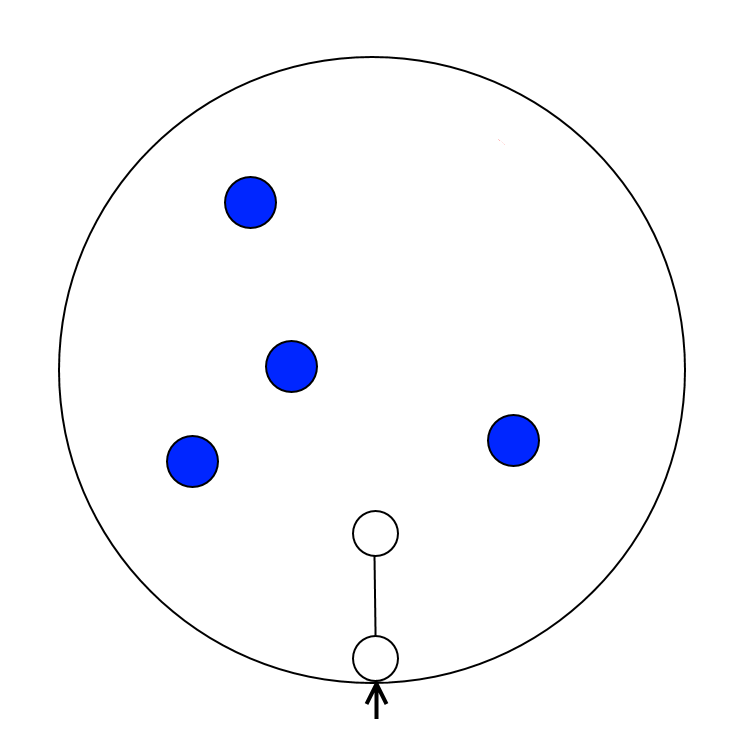
\includegraphics[height=.9\textheight]{images/CH3_SCA_Basic1.png}
\end{center}




\newpage
\begin{center}
	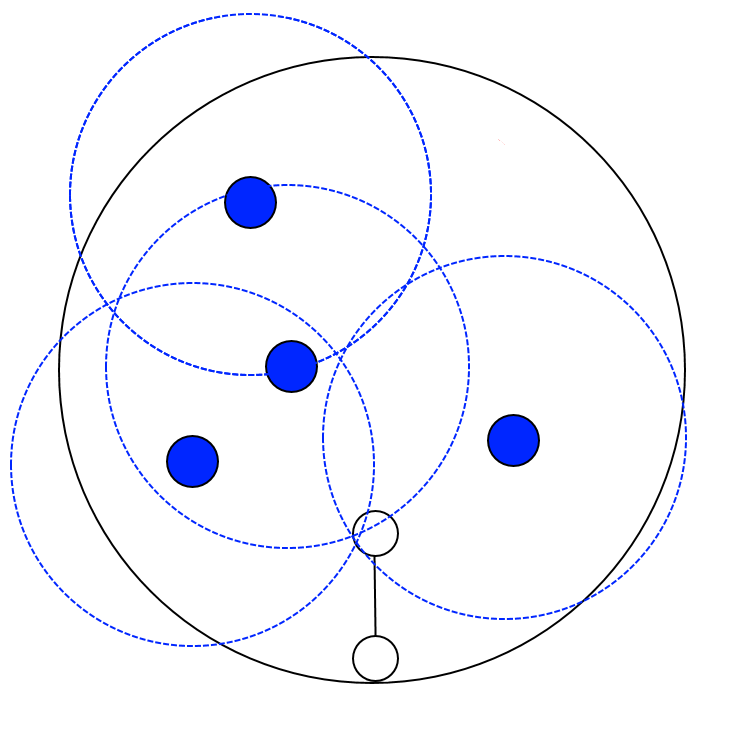
\includegraphics[height=.9\textheight]{images/CH3_SCA_Basic2.png}
	
	Bestimmung der minimal entfernten Knotenpunkte im Einflussradius
\end{center}





\newpage
\begin{center}
	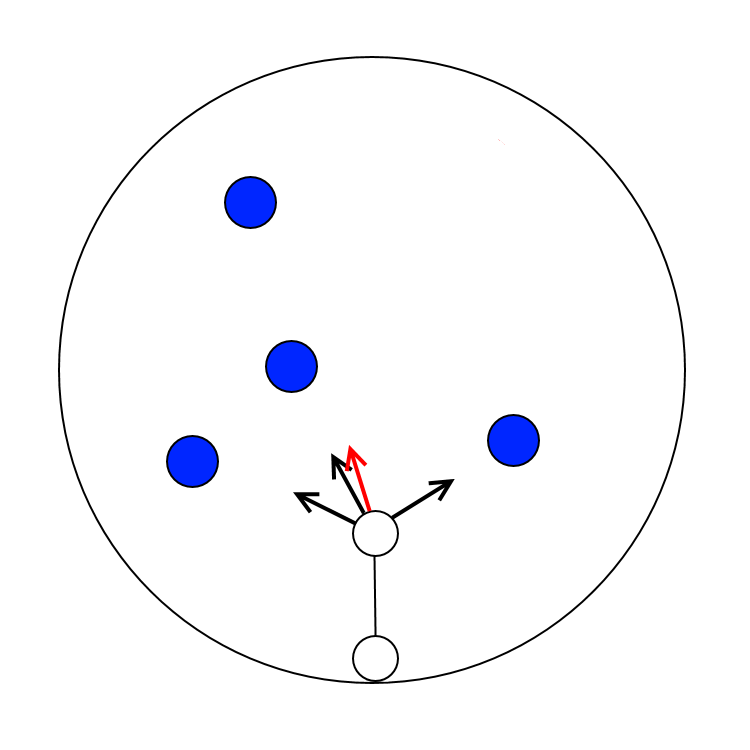
\includegraphics[height=.9\textheight]{images/CH3_SCA_Basic3.png}
	
	Berechnung der Wachstumsrichtung
\end{center}




\newpage
\begin{center}
	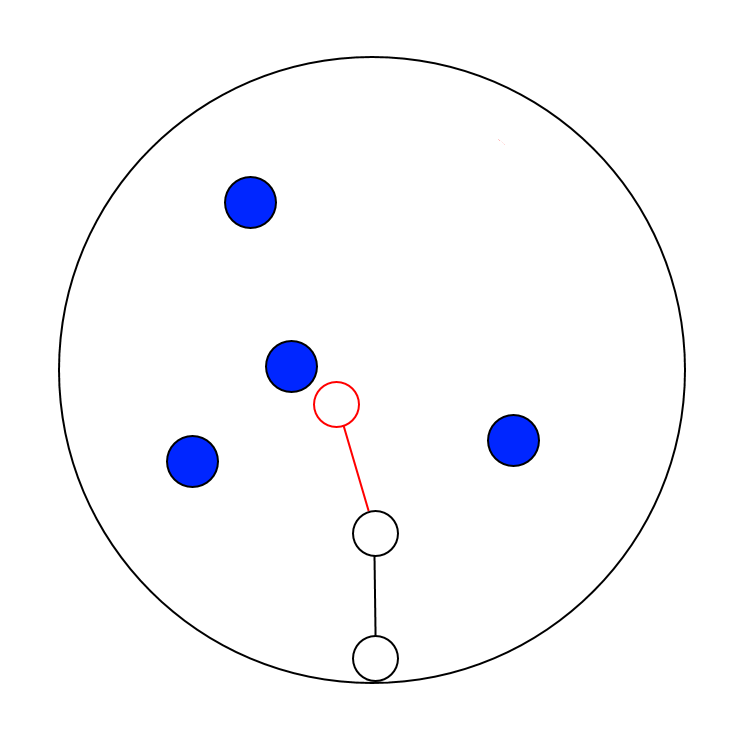
\includegraphics[height=.9\textheight]{images/CH3_SCA_Basic4.png}
	
	Platzierung des neuen Knotenpunkts
\end{center}




\newpage
\begin{center}
	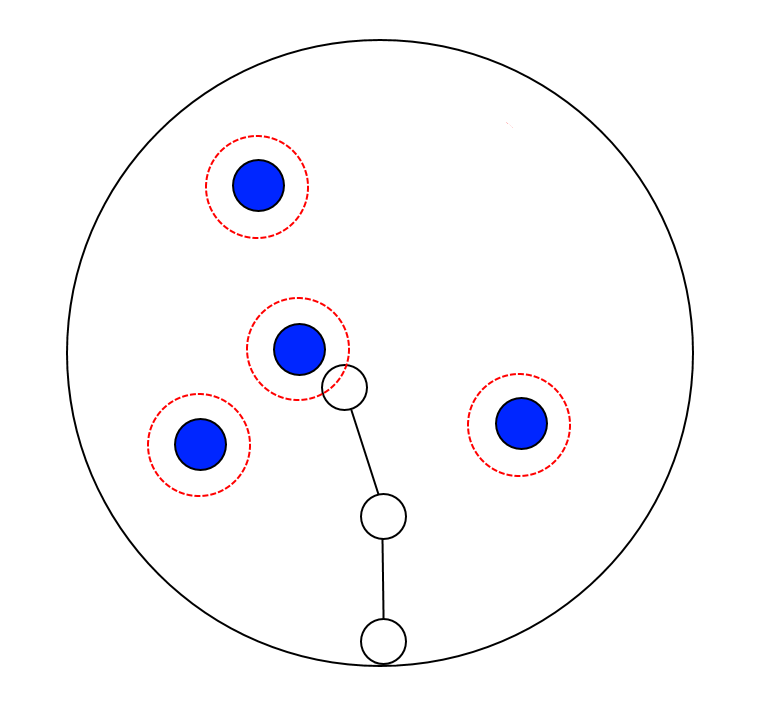
\includegraphics[height=.9\textheight]{images/CH3_SCA_Basic5.png}
	
	Bestimmung der Knotenpunkte im Minimalradius
\end{center}





\newpage
\begin{center}
	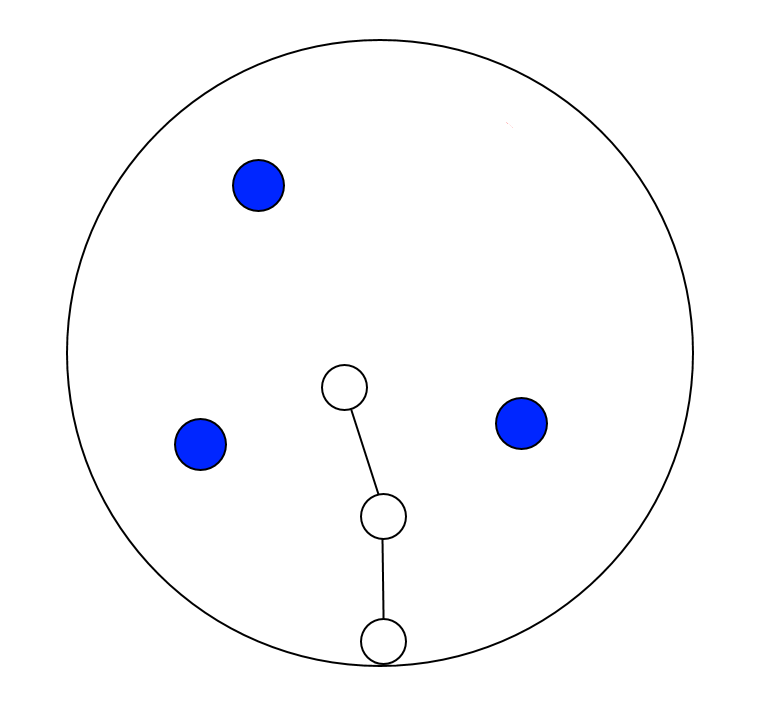
\includegraphics[height=.9\textheight]{images/CH3_SCA_Basic6.png}
	
	Ausgangssituation der nächsten Iteration
\end{center}




\newpage
\begin{center}
	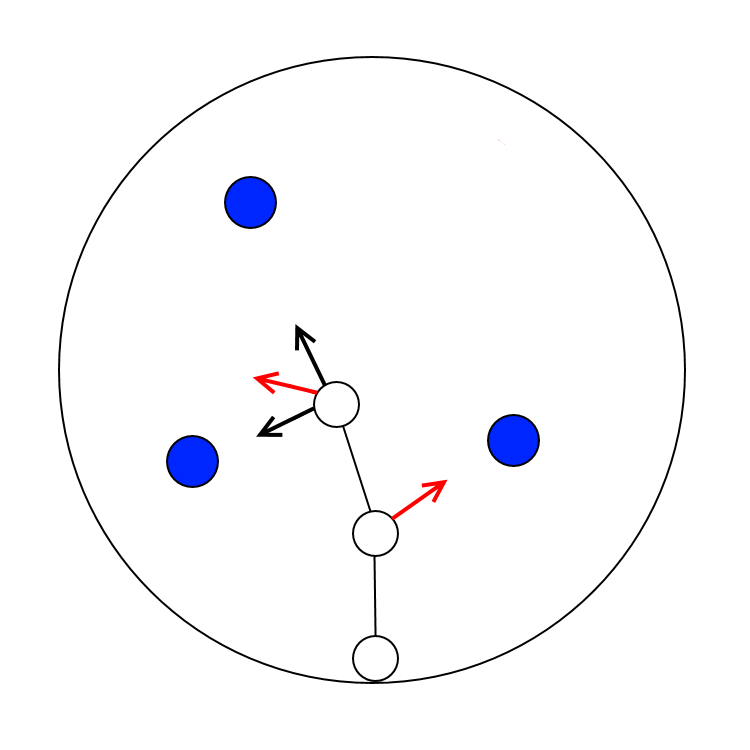
\includegraphics[height=.9\textheight]{images/CH3_SCA_Basic7.png}
	
	Beeinflussung unterschiedlicher Knotenpunkte
\end{center}




\newpage
\begin{center}
	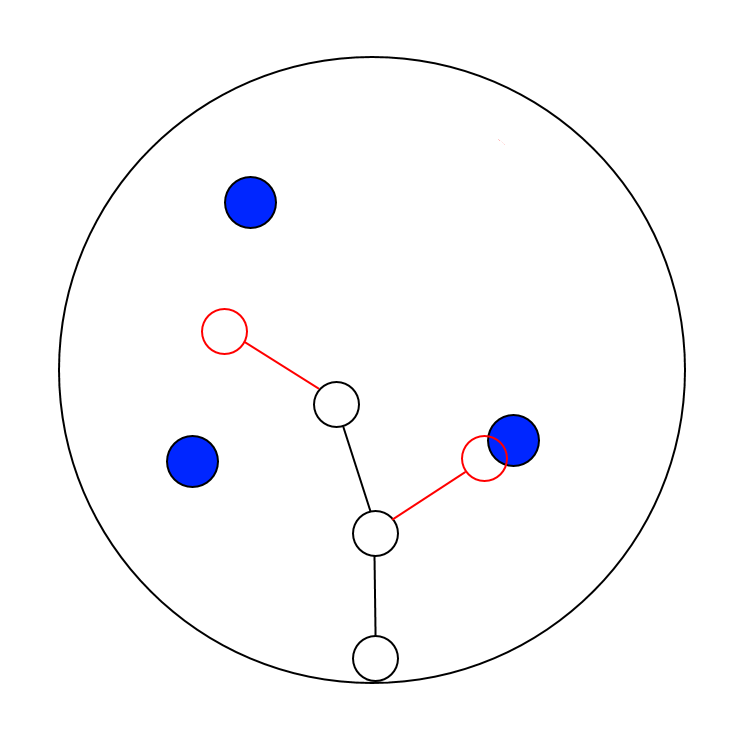
\includegraphics[height=.9\textheight]{images/CH3_SCA_Basic8.png}
	
	Entstehende Verzweigung
\end{center}




\newpage
\slidetitle{3. Space Colonization Algorithmus - Baumstrukturen}
\subsection{Generierung von Baumstrukturen\\}

\begin{enumerate}
	\item Befüllung des vorgegebenen Einflussbereichs\\
	
	\item Iterative Generierung\\
	
	\item Annäherung der Nachfolger jedes Knotenpunktes\\
	
	\item Visualisierung der Kanten mithilfe von Zylindern
\end{enumerate}





\newpage
\begin{center}
	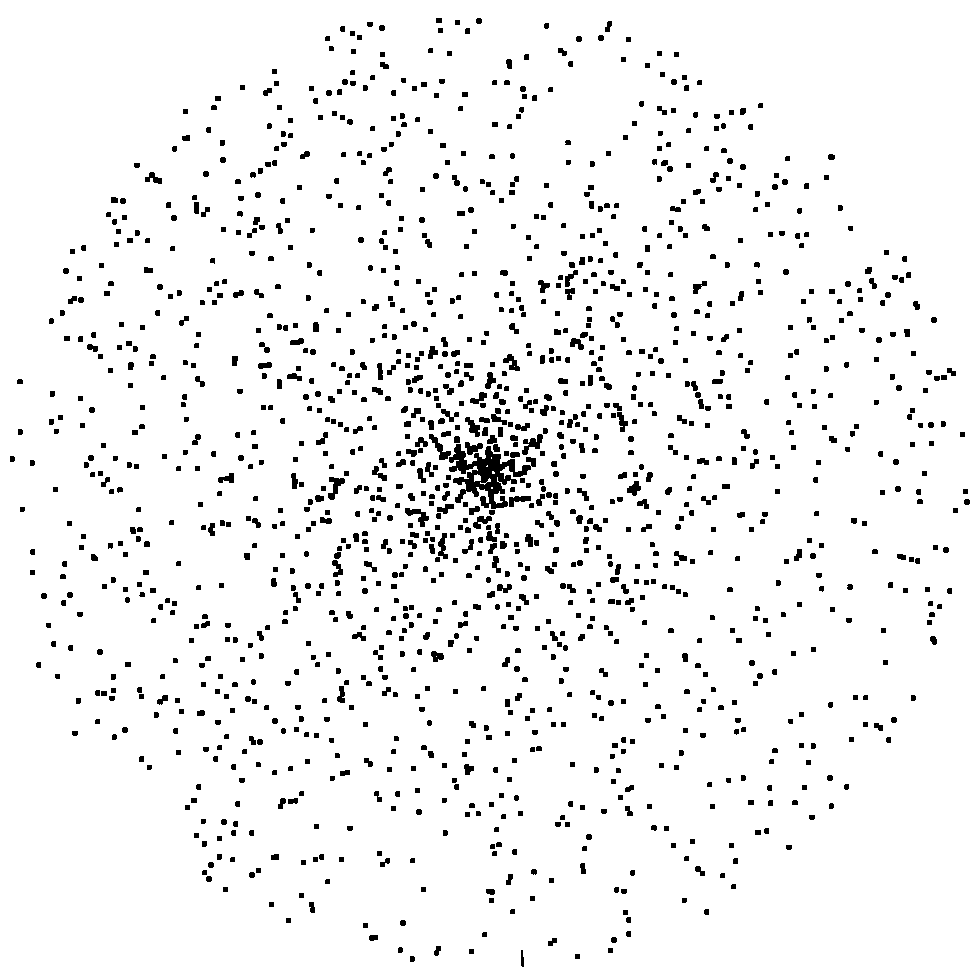
\includegraphics[height=.9\textheight]{images/CH3_SCA_Extended1.png}
	
	Verteilung von $2000$ Einflusspunkten in einem Rings mit Radius $r=500$
\end{center}





\newpage
\slidetitle{3. Space Colonization Algorithmus - Baumstrukturen}
\begin{center}
	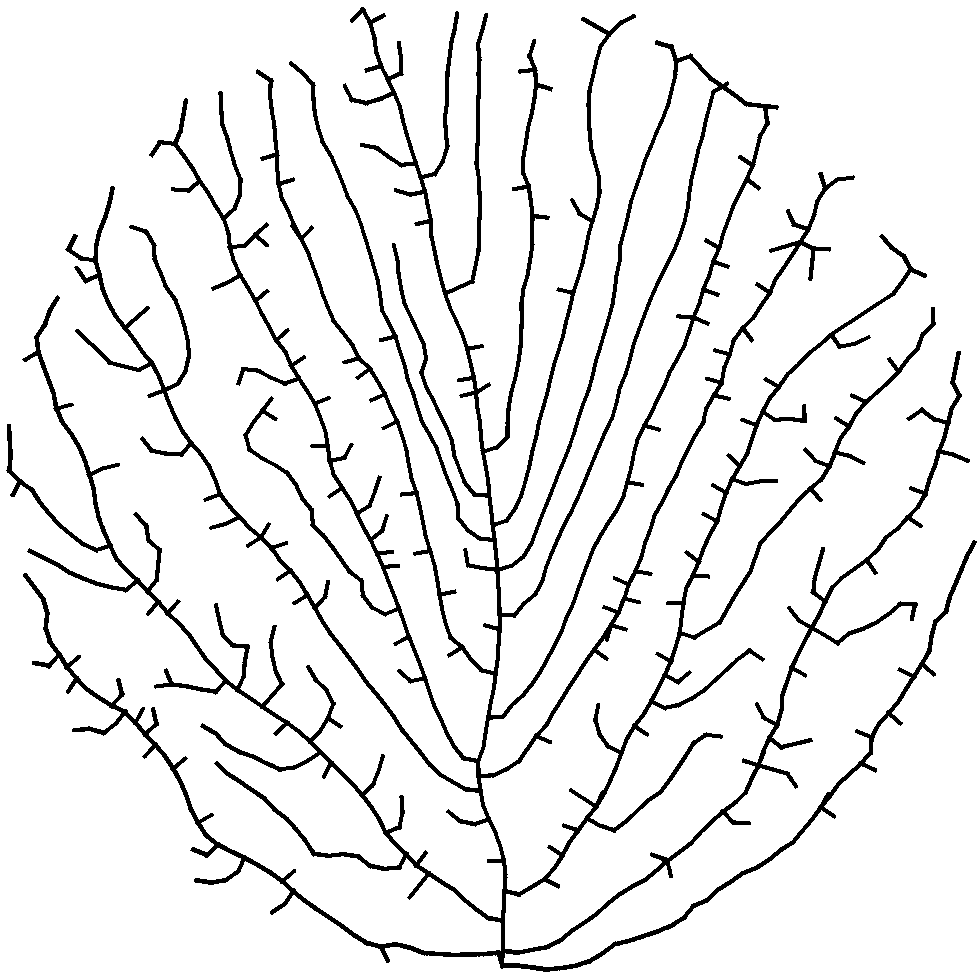
\includegraphics[height=.9\textheight]{images/CH3_SCA_Extended2.png}
	
	Ergebnis der iterativen Generierung	 mit $d_i = 100$, $d_k=20$, $D=15$, $\overrightarrow{T} = \overrightarrow{0}$			
\end{center}




\newpage
\slidetitle{3. Space Colonization Algorithmus - Baumstrukturen}
\begin{center}
	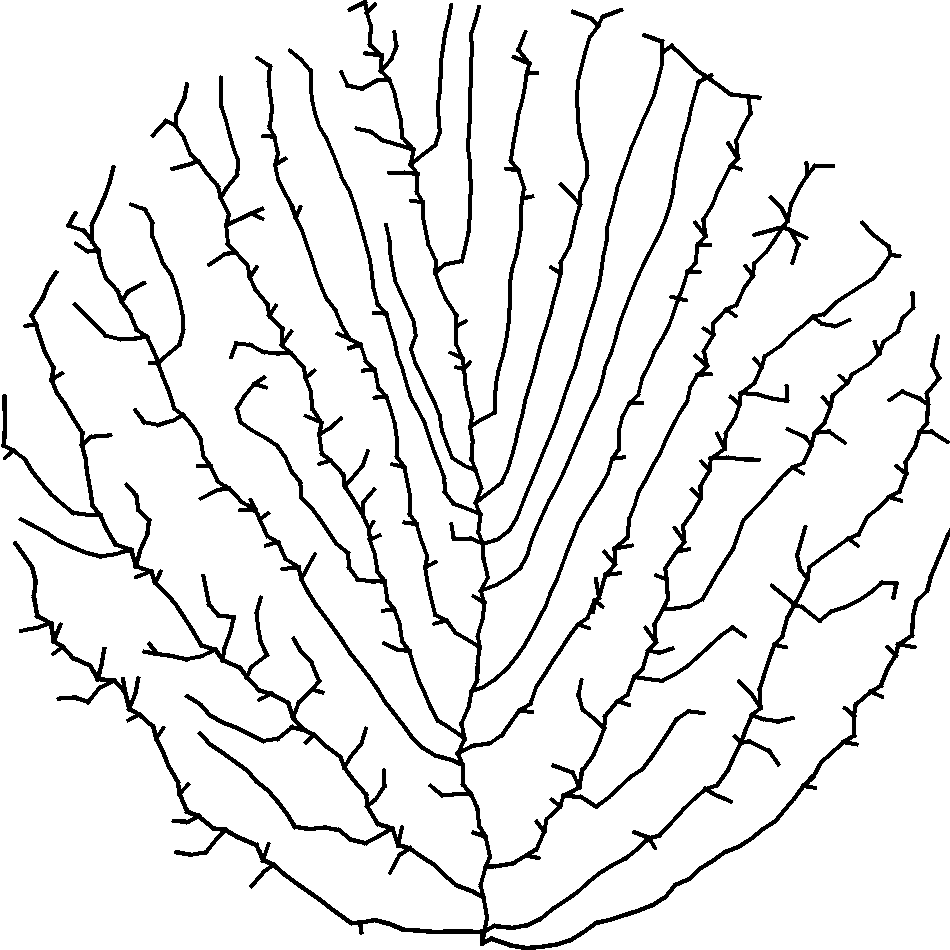
\includegraphics[height=.9\textheight]{images/CH3_SCA_Extended3.png}
	
	Annäherung der Nachfolger jedes Knotenpunktes
\end{center}





\newpage
\slidetitle{3. Space Colonization Algorithmus - Baumstrukturen}
\begin{center}
	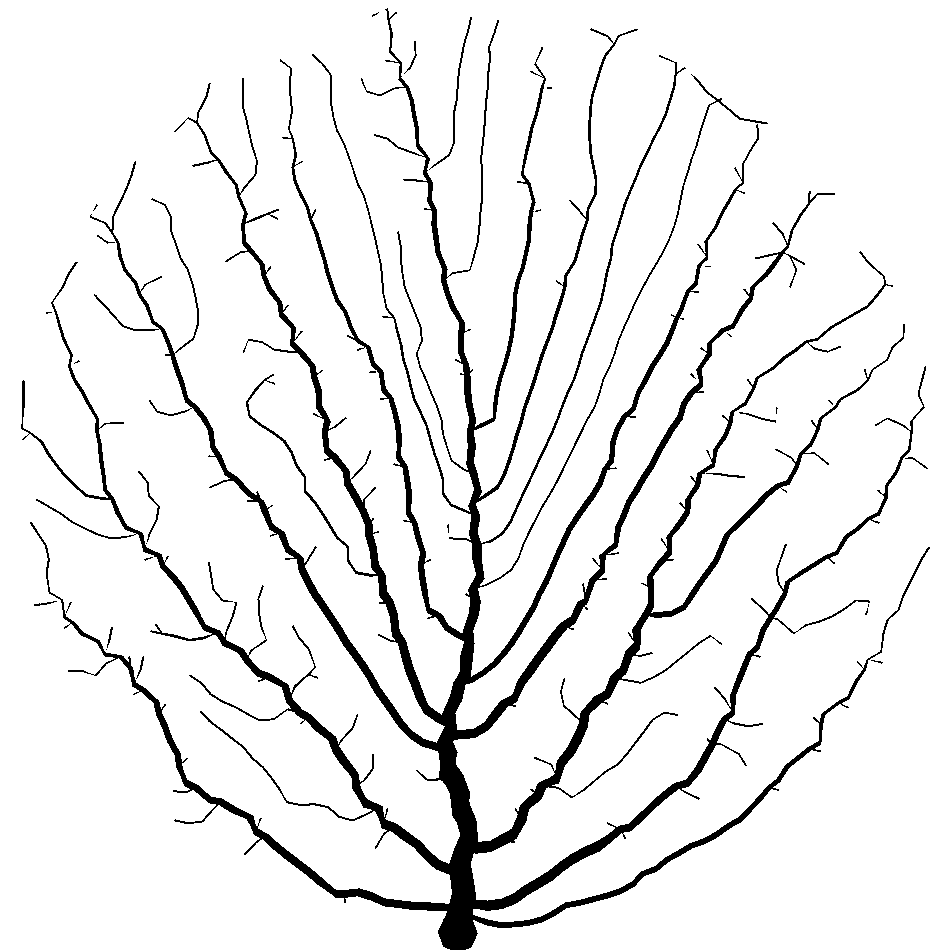
\includegraphics[height=.9\textheight]{images/CH3_SCA_Extended4.png}
	
	Visualisierung mithilfe von Zylindern
\end{center}




\iffalse
\newpage
\slidetitle{}
\subsection{Erweiterungen\\}

\begin{description}
	\item[\textbf{Zweigtiefe:}] Abhängig von der Anzahl an Verzweigungen\\
	
	\item[\textbf{Zusätzliche Bedingungen:}] Maximaler Grad, maximale Zweigtiefe, maximaler \glqq No-Growth\grqq -Wert\\
	
	\item[\textbf{Gewichtetes Wachstum:}] Erhöhung der Schrittweite in Abhängigkeit von der Zweigtiefe\\
	
	\item[\textbf{Kurvenreduktion:}] Eliminierung von Knoten in Abhängigkeit der Abzweigungswinkel\\
\end{description}





\newpage
\slidetitle{3. Space Colonization Algorithmus - Erweiterungen}
\fi